\documentclass[a4paper,10pt]{article}
\usepackage[utf8]{inputenc}
\graphicspath{{/home/robin/Dropbox/Thesis/Figures}} 
%opening
\usepackage{cleveref}
\usepackage{makeidx}
\usepackage{booktabs}
\usepackage{multirow}
\usepackage{threeparttable}
\makeindex
\usepackage[totoc]{idxlayout}

% Making R code work!
\usepackage{listings}
\usepackage{color}

\definecolor{dkgreen}{rgb}{0,0.6,0}
\definecolor{gray}{rgb}{0.5,0.5,0.5}
\definecolor{mauve}{rgb}{0.58,0,0.82}

\lstset{ %
  language=R,                % the language of the code
   basicstyle=\normalsize\ttfamily,           % the size of the fonts that are
% used for the code
% %   numbers=left,                   % where to put the line-numbers
% %   numberstyle=\tiny\color{gray},  % the style that is used for the
% line-numbers
% %   stepnumber=2,                   % the step between two line-numbers. If it's
% 1, each line
%                                   % will be numbered
% %   numbersep=5pt,                  % how far the line-numbers are from the code
% %   backgroundcolor=\color{white},      % choose the background color. You must
% add \usepackage{color}
% %   showspaces=false,               % show spaces adding particular underscores
% %   showstringspaces=false,         % underline spaces within strings
% %   showtabs=false,                 % show tabs within strings adding particular
% underscores
%    frame=false,                   % adds a frame around the code
%    rulecolor=\color{white},        % if not set, the frame-color may be changed
% on line-breaks within not-black text (e.g. commens (green here))
% %   tabsize=2,                      % sets default tabsize to 2 spaces
% %   captionpos=b,                   % sets the caption-position to bottom
% %   breaklines=true,                % sets automatic line breaking
% %   breakatwhitespace=false,        % sets if automatic breaks should only
% happen at whitespace
% %   title=\lstname,                   % show the filename of files included with
\lstinputlisting;
                                  % also try caption instead of title
  keywordstyle=\color{blue},          % keyword style
  commentstyle=\color{dkgreen},       % comment style
  stringstyle=\color{mauve},         % string literal style
  escapeinside={\%*}{*)},            % if you want to add a comment within your
% code
  morekeywords={*,...}               % if you want to add more keywords to the
% set
}

% Include any extra LaTeX packages required
\usepackage[round,]{natbib}  % Use the "Natbib" style for the references
\usepackage{verbatim}  % Needed for the "comment" environment to make LaTeX
comments
\hypersetup{urlcolor=blue, colorlinks=false}  % 
\title{}
\author{}

\begin{document}

\maketitle

\begin{abstract}

\end{abstract}

\subsection{IPF theory: a worked example} \label{s:theory}
In most modelling texts there is a strong precedence of theory over
application: the latter usually flows from the former. The
location of this section after a description of the programming language
R is therefore
slightly unconventional. There is a logic to this order however: now that we
understand something (the power and flexibility) of the programming language in
which the model is written, the next stage is to analyse the task to which it
is to be set. More importantly for reproducible research, this theory section
is illustrated with a simple worked example that culminates in
a question to the reader, to test his or her understanding.
In section after this one, we will show how these same calculations can be
automated in R (\cref{simplementing}, using the same example dataset
(which is also replicated in an `rpubs' document,
\href{http://rpubs.com/RobinLovelace/6193}{available online}).

This decision is not designed to downplay the importance of pure theory, which
is still best pursued in the language of pure mathematics. However,
our concern here is not the development of new theory --- this has been dealt
with in key papers on the subject such as \citep{Williamson1998},
\citep{Pritchard2012} and
others referenced in \cref{Chapter3} --- but
the application of existing theory.

IPF produces maximum likelihood estimates of spatially
disaggregated conditional probabilities for the individual attributes of
interest.
The method is also known as `matrix raking', RAS
or `entropy maximising'
(see \citealp{Johnston1993, Birkin1988, Muller2010, Huang2001a,
Simpson2005, Kalantari2008, Jirousek1995}).
The mathematical properties of IPF
have have been described in several papers
(see for instance \citealp{Bishop1975, Fienberg1970, Birkin1988}).
Illustrative examples of the procedure can be found in
\citet{Saito1992}, \citet{Wong1992}
and \citet{Norman1999a}.
\citet{Wong1992} investigated the reliability of IPF and evaluated
the importance of different factors influencing the its performance.
Similar methodologies have since been employed by
\citet{Mitchell2000}, \citet{Williamson2002} and
Ballas et al.~\citeyearpar{Ballas2005c, Ballas2005}
to investigate a wide range of phenomena.

% As \citet{Birkin1988} point out, IPF undertakes the basic task of
% generating a vector of individual characteristics, $x = (x_1, x_2, ..., x_m)$
on the
% basis of a joint probability distribution $p(x)$. Once the probability
distribution
% for such a vector is generated, representative
% individuals can be synthesised or extracted from a pre-existing survey
dataset.
% However, when information is not available for the full joint distribution,
there
% is a need to construct a product of conditional and marginal probabilities,
% by building one attribute at a time, so that the probability of certain
attributes
% is conditionally dependent on existing attributes \citep{Birkin1988}:
%
% \begin{equation}
% p(x) = p(x_1)p\left( \frac{x_2}{x_1}\right) p\left( \frac{x_3}{x_2},
x_1\right) \times
%  ... \times p\left( \frac{x_m}{x_{m-1}},...,x_1\right)
% \end{equation}
%
% IPF can be used to model the joint probability distribution
% $p(x_1, x_2, x_3)$ subject to known probabilities
% $p(x_1, x_2)$ and $p(x_1, x_3)$. Following \citet{Birkin1988} and
\citet{Ballas2007simb},
% if $p(x_1, x_2, x_3)$ is the $i^{th}$ approximation to the three-attribute
joint probability
% vector then:
% \begin{equation}
%  p^1(x_1, x_2, x_3) = \frac{1}{N_1 N_2 N_3}
% \end{equation}
% where $N_j$ is the number of possible states associated with the attribute
vector $x$.
% The vector can then be adjusted in \emph{proportion} to the following known
constraints:
% \begin{equation}
% p^2(x_1, x_2, x_3) = p^1(x_1, x_2, x_3) \frac{p(x_1, x_2)}
% {{\displaystyle \sum^{}_{x_3}{p^1(x_1, x_2, x_3)}}}
% \label{eq:p2}
% \end{equation}
% \begin{equation}
% p^3(x_1, x_2, x_3) = p^2(x_1, x_2, x_3) \frac{p(x_1, x_3)}
% {{\displaystyle \sum^{}_{x_2}{p^1(x_1, x_2, x_3)}}}
% \label{eq:p3}
% \end{equation}
% IPF involves iterating through equations \ref{eq:p2} and \ref{eq:p3}
% until a \emph{fitted} distribution is obtained, when the probabilities
% are convergent within some acceptable limit \citep{Birkin1988, Fienberg1970,
Ballas2007simb}.
% This procedure can be generalised to a larger number of attributes
\citep{Birkin1988}:
% if we let $Z_k(x)$ be a subset of the set of attribute vectors
% $E(x)$ for which marginal joint probabilities are known and let $W_k(x)$ be
% the complement of $Z_k(x)$, that is $W_k(x)= E(x) - Z_k(x)$, then:
%
% \begin{equation}
%  p^1(x) = \frac{1}{\displaystyle{\prod^{m}_{i=1}{Ni}}}
% \end{equation}
% \begin{equation}
%  p^2(x) =  p^1(x) \frac{p[Z_1(x)]}{\displaystyle{\sum^{}_{W_1(x)}{p^1(x)}}}
% \label{eq:six}
% \end{equation}
%
% {\centering
% .
%
% .
%
% .
%
% }
%
% \begin{equation}
%  p^{k+1}(x) =  p^k(x)
\frac{p[Z_k(x)]}{\displaystyle{\sum^{}_{W_k(x)}{p^k(x)}}}
% \label{eq:seven}
% \end{equation}
%
% IPF iterates through equations \ref{eq:six} and \ref{eq:seven} until
convergence
% \citep{Birkin1988}. An extensive discussion of the mathematical properties of
% IPF can be found in \citet{Fienberg1970}.

To illustrate how IPF works in practice, a simplified example is described
below.
This is a modified version of a simpler demonstration from
\citet{Ballas2005}.\footnote{In \citet{Ballas2005}
the interaction between the age and sex constraints are assumed to be known.
(Their equivalent of \cref{t:s2} contains data for every cell,
not question marks.) This results in IPF converging instantly.
However, in Census data, such cross-tabulation is
often absent, and IPF must converge over multiple constraints and
iterations. This latter scenario is assumed in the worked example below.}
Table \ref{t:w}  describes a
hypothetical microdataset comprising 5 individuals, who are defined by two
constraint variables, age and sex. Each has two categories.
Table \ref{t:s} contains aggregated data
for a hypothetical area, as it would be download from census dissemination
portal Casweb. \Cref{t:s2} illustrates this table in a different form,
which shows our ignorance of interaction between age and sex.


\begin{table}[h]
\centering
\caption{A hypothetical input microdata set (the original
weights set to one). The bold value is used subsequently for
illustrative purposes.}
\begin{tabular}{llll}
\toprule
{Individual } & {Sex} & {Age-group} & {Weight} \\
\midrule
1 & Male & Over-50 & 1 \\
2 & Male & Over-50 & 1 \\
3 & {Male} & {Under-50} & \textbf{1} \\
4 & Female & Over-50 & 1 \\
5 & Female & Under-50 & 1 \\
\bottomrule
\end{tabular}
\label{t:w}
\end{table}
\vspace{1cm}


\begin{table}[htbp]
\centering
\caption{Hypothetical small area constraints data ($s$).}
\begin{tabular}{cllll}
\toprule
Constraint $\Rightarrow$ & \multicolumn{2}{c}{$i$}& \multicolumn{2}{c}{$j$}\\
Category $\Rightarrow$ & $i_1$ & $i_2$ & $j_1$ & $j_2$ \\
Area $\Downarrow$  & Under-50 & Over-50 &  Male & Female\\
1  & 8 & 4 & 6 & 6\\
\bottomrule
\end{tabular}
\label{t:s}
\end{table}
\vspace{1cm}

\begin{table}[htbp]
\centering
\caption{Small area constraints expressed as marginal totals, and the cell
values to be estimated.}
\begin{tabular}{cllll}\toprule
Marginal totals&  & \multicolumn{2}{c}{$j$} & \\
& Age/sex & Male & Female & T\\ \midrule
\multirow{2}{*}{$i$} & Under-50 & \textbf{?} & ? & 8\\
& Over-50 & ? & ? &4 \\
& T & 6 & 6 &12\\
\bottomrule
\end{tabular}
\label{t:s2}
\end{table}

Table \ref{t:m} presents the
hypothetical microdata in aggregated form,
that can be compared directly to Table \ref{t:s2}.

\begin{table}[htbp]
\centering
\caption{The aggregated results of the weighted
microdata set ($m(1)$).
Note, these values depend on the
weights allocated in Table \ref{t:w} and therefore
 change after each iteration}

\begin{tabular}{cllll}\toprule
Marginal totals&  & \multicolumn{2}{c}{$j$} & \\
& Age/sex & Male & Female & T\\ \midrule
\multirow{2}{*}{$i$} & Under-50 & \textbf{1} & 1 & 2\\
& Over-50 & 2 & 1 &3 \\
& T & 3 & 2 &5\\
\bottomrule
\end{tabular}
\label{t:m}
\end{table}

Using these data it is possible to readjust the weights of the hypothetical
individuals, so that their sum would add up to the totals given in Table
\ref{t:s2} (12). In particular, the weights can be readjusted by multiplying
them by
the marginal totals, originally taken from
Table \ref{t:s} and then divided by the respective marginal total in \ref{t:m}.
Because the total for each small-area constraint is 12, this must be
done one constraint at a time. This
can be expressed, for a given area and a given constraint ($i$
or age in this case), as follows:

\begin{equation}
w(n+1)_{ij} = \frac{w(n)_{ij} \times sT_{i}}{mT(n)_{i}}
\label{eq:ipf}
\end{equation}
where $w(n+1)_{ij}$ is the new weight for individuals with characteristics $i$
(age, in this case), and $j$ (sex),  $w(n)_{ij}$ is the original
weight for individuals with these characteristics, $sT_{i}$ is element
marginal total of the small area constraint, $s$
(Table \ref{t:s}) and $mT(n)_{i}$ is the marginal total of category
$j$ of the aggregated results of the weighted
microdata, $m$ (Table \ref{t:m}). $n$ represents the iteration number.
Although the marginal totals of $s$ are known, its cell values
are unknown. Thus, IPF estimates the interaction (or cross-tabulation)
between constraint variables.
(Follow the emboldened values in the tables
to see how the new weight of individual 3 is calculated for the sex constraint.)
Table \ref{t:new-weights} illustrates the weights that result. Notice that the
sum of the weights is equal to the total population, from the constraint
variables.

\begin{table}[htbp]
\centering
\caption{Reweighting the hypothetical microdata set in order to fit
Table \ref{t:s}.}
\begin{tabular}{lllll}
\toprule
{Individual} & {Sex} & {age-group} & {Weight} &
{New weight, w(2)} \\ \midrule
1 & Male & Over-50 & 1 & $1 \times 4/3 = \frac{4}{3}$ \\
2 & Male & Over-50 & 1 & $1 \times 4/3 = \frac{4}{3}$ \\
3 & Male & Under-50 & 1 & $\textbf{1} \times
\textbf{8}/\textbf{2} = 4$ \\
4 & Female & Over-50 & 1 & $1 \times 4/3 = \frac{4}{3}$ \\
5 & Female & Under-50 & 1 & $1 \times 8/2 = 4$ \\
\bottomrule
\end{tabular}
\label{t:new-weights}
\end{table}

After the individual-level data has been re-aggregated (\cref{t:m2}),
the next stage is to repeat \cref{eq:ipf} for the age constraint to generate a
third set of weights, by replacing
the $i$ in $sT_{i}$ and $mT(n)_{i}$ with $j$ and incrementing the value of n:

\begin{equation}
w(3)_{ij} = \frac{w(2)_{ij} \times sT_{j}}{mT(2)_{j}}
\label{eq:ipf2}
\end{equation}

To test your understanding of IPF, apply \cref{eq:ipf2} to the information above
and that presented in \cref{t:m2}.
This should result in the following vector of new weights, for individuals 1 to
5:
\begin{equation}
 w(3) = (\frac{6}{5}, \frac{6}{5}, \frac{18}{5}, \frac{3}{2}, \frac{9}{2})
\end{equation}
As before, the sum of the weights is equal to the population of the area (12).
Notice also that after each iteration the fit between the marginal
totals of $m$ and $s$
improves. The total absolute error (TAE, see \cref{etae} below)
from $m(1)$ to $m(2)$ improves from
14 to 6 in \cref{t:m} and \cref{t:m2} above. TAE for $m(3)$ (not shown,
but calculated by aggregating $w(3)$) improves even more, to 1.3.
This number would eventually converge to 0 through subsequent
iterations, as there are no empty cells in the input microdataset;
a defining feature of IPF.


\begin{table}[htbp]
\centering
\caption{The aggregated results of the weighted
microdata set after constraining for age ($m(2)$).
}

\begin{tabular}{cllll}\toprule
Marginal totals&  & \multicolumn{2}{c}{$i$} & \\
& Age/sex & Male & Female & T\\ \midrule
\multirow{2}{*}{$j$} & Under-50 & 4 & 4 & 8\\
& Over-50 & $\frac{8}{3}$ & $\frac{4}{3}$ & 4 \\
& T & $6\frac{2}{3}$ & 5$\frac{1}{3}$ & 12\\
\bottomrule
\end{tabular}
\label{t:m2}
\end{table}

The above process, when applied to more categories (e.g. socio-economic class)
and repeated iteratively until a satisfactory convergence occurs, results in a
series of weighted microdatasets, one for each of the small areas being
simulated. This allows for the estimation of variables whose values are not
known at the local level (e.g. income) \citep{Ballas2005}. An issue
with the results of IPF (absent from combinatorial optimisation methods),
however, is that it results in non-integer weights: fractions of individuals
appear in simulated areas. As described in the introduction, this is not ideal
for certain applications. Integer weights allow the results of spatial
microsimulation to be further processed using dynamic microsimulation and agent
based modelling techniques \citep{Pritchard2012}.


% A key benefit from a policy perspective is that
% IPF and other spatial microsimultion techniques
% can provide estimation of variables whose values are not
% known at the local level (e.g. income).
Spatial microsimulation can also provide insight into the likely
distribution of individual-level variables about which only
geographically aggregated statistics have been made available.
An issue
with the results of IPF (absent from combinatorial optimisation methods),
however, is that it results in non-integer weights: fractions of individuals
appear in simulated areas.

\subsection{Implementing IPF in R} \label{simplementing}
The above example is best undertaken by hand, probably with a pen and paper
to gain an understanding of IPF. To do the calculations for a larger
dataset would clearly be a waste of time, as computers have been developed
to automate repetitive calculations. This section explains how the IPF
algorithm described above was implemented in R, using a slightly more
complex example. This section is based on ``Spatial microsimulation in R: a
beginner’s guide to iterative proportional fitting (IPF)'', a tutorial
written to accompany a methods paper on integerisation
\citep{}.\footnote{This tutorial is available from Rpubs, a site dedicated
to publishing R analyses that are reproducible. It uses the RMarkdown
mark-up language, which enables R code to be run and presented within
documents. See http://rpubs.com/RobinLovelace/5089 \label{fnrpub} .}

\emph{Loading in the data}

In the full model the input datasets are stored as .csv files, one for each
constraint and one for the input microdata, and read in with the command
\verb read.csv . For the purposes of this understanding how the model works,
however, we will type-in the data line by line, following-on from the
example above. The following code creates example datasets,
based on the same hypothetical survey of 5 individuals described above,
and 5 small areas. The spatial microsimulation model will select individuals
based on age and sex and mode of transport (mode of transport
is also used on the larger online example described in footnote \ref{fnrpub}).
For consistency with the (larger) model used for the paper, we will refer to
the individual-level data as USd (short for Understanding Society dataset)
and the geographic data as all.msim (for all constraint variables).
Code to read-in the individual-level data is presented in code sample
\ref{cusd}.
When called, the data is then displayed as a table (see listing \ref{cout}).
\begin{lstlisting}[float=h, caption={Manual input of individual-level data
in R}, label=cusd]
# Read in the data in long form (normaly read.table() used)
c.names <- c("id", "age", "sex")
USd <- c(       1, 59, "m",
                2, 54, "m",
                3, 35, "m",
                4, 73, "f",
                5, 49, "f")
USd <- matrix(USd, nrow = 5, byrow = T) # Long data into matrix
USd <- data.frame(USd) # Convert this into a dataframe
names(USd) <- c.names # Add correct column names
USd$age <- as.numeric(levels(USd$age)[USd$age]) # Age is a numeric
\end{lstlisting}
\begin{lstlisting}[float=h, caption={Output of the USd data frame}, label=cout]
USd # Show the data frame in R
##   id age sex
## 1  1  59   m
## 2  2  54   m
## 3  3  35   m
## 4  4  73   f
## 5  5  49   f
\end{lstlisting}
The same procedure applies to the geographical data (listing \ref{cgeo}).
\begin{lstlisting}[float=h*, caption={Geographic data input}, label=cgeo]
 category.labels <- c("16-49", "50+" # Age constraint
             ,"m", "f" # Sex constraint
             # more constraints could go here
             )
all.msim <- c(  8, 4,    6, 6,   # Original aggregate data
                2, 8,    4, 6,   # Elderly
                7, 4,    3, 8,   # Female dominated
                5, 4,    7, 2,   # Male dominated
                7, 3,    6, 4    # Young
                )
all.msim <- matrix(all.msim, nrow = 5, byrow = T)
all.msim <- data.frame(all.msim) # Convert to dataframe
names(all.msim) <- category.labels # Add correct column names
\end{lstlisting}

IPF relies on the assumption that all constraint variables will contain the
same number of people. This is logical (e.g.~how can there be more people
classified
by age than by sex?) but can cause problems for constraint variables that use
only a subset of the total population, such as those who responded to questions
on
travel to work. To overcome this problem, it is possible to normalise the
constraint variables, setting the total for each to the one that has the most
reliable total population. In this worked example, we simply check whether
or not they are (listing \ref{ccheck}).

\begin{lstlisting}[float=h, caption={R code to check the constrain populations
match}, label=ccheck]
 # Check totals for each constraint match
rowSums(all.msim[,1:2]) # Age constraint
## [1] 12 10 11  9 10
rowSums(all.msim[,3:4]) # Sex constraint
## [1] 12 10 11  9 10

rowSums(all.msim[,1:2]) == rowSums(all.msim[,3:4])
## [1] TRUE TRUE TRUE TRUE TRUE
\end{lstlisting}

\emph{Reweighting the survey dataset}

Iterative proportional fitting determines the weight allocated to each
individual for each zone to best match the geographically aggregated data.
A weight matrix is therefore created, with rows corresponding to individuals
and columns to zones, as described \cref{s:theory} as a vector. In
R, this, and the creation of the aggregated results matrix,
is done with code presented in listing
\ref{cws}).\footnote{In subsequent
versions of the model, single, multi-dimensional weight and
aggregated result matrices are used,
to reduce the length of the scripts.
}

\begin{lstlisting}[float=h, caption={Creating arrays of weights in R},
label=cws]
weights0 <- array(dim=c(nrow(USd),nrow(all.msim)))
weights1 <- array(dim=c(nrow(USd),nrow(all.msim)))
weights2 <- array(dim=c(nrow(USd),nrow(all.msim)))

weights0[,] <- 1 # sets initial weights to 1

USd.agg <- array(dim=c(nrow(all.msim),ncol(all.msim)))
USd.agg1 <- array(dim=c(nrow(all.msim),ncol(all.msim)))
USd.agg2 <- array(dim=c(nrow(all.msim),ncol(all.msim)))
colnames(USd.agg1) <- category.labels
\end{lstlisting}

It important to note that in real survey data, the variables are not
always neatly categorised into the same bins as the levels of the aggregate
data. Age, for example can be classified in many different ways.
Also, a wide form is useful for subsequent steps.
Therefore, it is necessary to convert the `thin' survey dataset
into a wider form, by converting a single column such as age or sex into
multiple columns corresponding to the number of categories. Sometimes the
cut-off points of the categories can be decided (as with age), or categories
can be merged (when many different NA options are available, for example).
The code that performs this important process for our example dataset is
presented in listing \ref{ccat}.

\begin{lstlisting}[float = h, caption={R code to convert the survey
dataset into binary form}, label=ccat]
USd.cat <- array(rep(0), dim=c(nrow(USd),
			  length(category.labels !=0)))

USd.cat[which(USd$age < 50),1] <- 1 # Age, "< 50"
USd.cat[which(USd$age >= 50),2] <- 1 # "50+"
USd.cat[which(USd$sex =="m"),3] <- 1 # Sex constraint: "m"
USd.cat[which(USd$sex =="f"),4] <- 1 #"f"
sum(USd.cat) # Should be 10
\end{lstlisting}

Another important step shown in \cref{s:theory} was that of converting the
`long' survey dataset into a form that can be compared directly with the
aggregated constraint variables. Listing \ref{cconv} shows how this is done
in R, and the code needed to view the results. (Notice that the first row
of all.msim is the same as those displayed in \cref{t:s})

\begin{lstlisting}[float=h, caption={R code to aggregate the survey dataset},
label=cconv]
 for (i in 1:nrow(all.msim)){ # Loop creating aggregate values
  USd.agg[i,]   <- colSums(USd.cat * weights0[,i])
}

# Test results
USd.agg

##      [,1] [,2] [,3] [,4]
## [1,]    2    3    3    2
## [2,]    2    3    3    2
## [3,]    2    3    3    2
## [4,]    2    3    3    2
## [5,]    2    3    3    2

all.msim

##   16-49 50+ m f
## 1     8   4 6 6
## 2     2   8 4 6
## 3     7   4 3 8
## 4     5   4 7 2
## 5     7   3 6 4

plot(as.vector(as.matrix(all.msim)),
  as.vector(as.matrix(USd.agg)), xlab = "Constraints",
    ylab = "Model output")
abline(a = 0, b = 1)
\end{lstlisting}

With the data loaded and processed into comparable formats, we are in a
position to start comparing how well our individual-level survey dataset
fits with the aggregate constraints (see listing \ref{cconv}). Note that for
USd.agg,
the results are the same for every zone, as each individual has a weight of 1
for every zone. Note also the very poor fit between the variables at the
aggregate level, as illustrated by poor correlation between the constraint and
microdata variables (r = 0.05), and a plot of the fit presented in \cref{fct1}.
The next stage is to apply the first constraint,
to adjust the weights of each individual so they match the age constraints
(listing \ref{ccon1} --- note that the top row USd.agg1 is the same as
\cref{t:m2}). After this operation, the fit between the constraint
variables and the aggregated microdata are far better (r = 0.67), but there
is still a large degree of error (\cref{fc1}).

\begin{figure}[h]
 \begin{center}
   
\includegraphics[width = 10cm]{unnamed-chunk-5}
 \end{center}
\caption[Scatter plot of the fit between census and survey data]
{Scatter plot of the fit between census and survey data. This plot
can be re-created using the plot command in listing \ref{cconv}}
 \label{fct1}
\end{figure}

\begin{lstlisting}[float=h, caption={Re-weighting of first constraint
and testing of results}, label=ccon1]
for (j in 1:nrow(all.msim)) {
    weights1[which(USd$age < 50), j] <- all.msim[j, 1]/USd.agg[j, 1]
    weights1[which(USd$age >= 50), j] <- all.msim[j, 2]/USd.agg[j, 2]
}
# Aggregate the results for each zone
for (i in 1:nrow(all.msim)) {
    USd.agg1[i, ] <- colSums(USd.cat * weights0[, i] * weights1[, i])
}
# Test results
USd.agg1
##      16-49 50+     m     f
## [1,]     8   4 6.667 5.333
## [2,]     2   8 6.333 3.667
## [3,]     7   4 6.167 4.833
## [4,]     5   4 5.167 3.833
## [5,]     7   3 5.500 4.500

plot(as.vector(as.matrix(all.msim)),
    as.vector(as.matrix(USd.agg1)), xlab = "Constraints",
    ylab = "Model output")
abline(a = 0, b = 1)
\end{lstlisting}

\begin{figure}[h]
 \begin{center}
  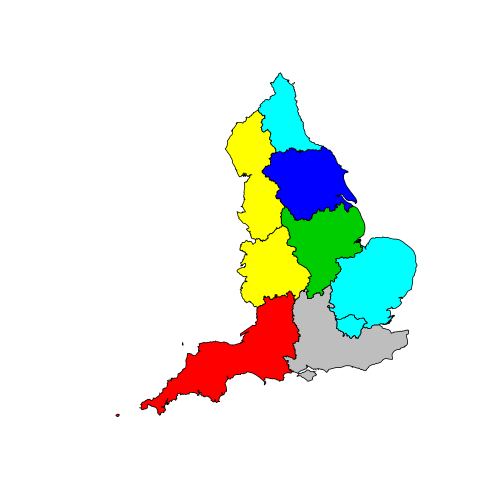
\includegraphics[width=10cm]{unnamed-chunk-6}
 \end{center}
\caption{Scatter plot showing the fit after constraining by age} \label{fc1}
\end{figure}

We will perform the same checks after
each constraint to ensure our model is improving.
To see how the weights change for each individual for each area,
we simply type \verb weights1 , for constraint 1 (listing \ref{cmat}).
(Note that the first column of weights 1 is the same as \cref{t:s}.)
\begin{lstlisting}[caption = {The new weight matrix (previously just ones)},
label =cmat]
 weights1
##       [,1]  [,2]  [,3]  [,4] [,5]
## [1,] 1.333 2.667 1.333 1.333  1.0
## [2,] 1.333 2.667 1.333 1.333  1.0
## [3,] 4.000 1.000 3.500 2.500  3.5
## [4,] 1.333 2.667 1.333 1.333  1.0
## [5,] 4.000 1.000 3.500 2.500  3.5
\end{lstlisting}

To further improve the fit, we constrain by the second aggregate constraint:
sex (listing \ref{con2}). To check that our implementation in R produces the
same results as the hand-calculated example, we queried the resulting weights.
As shown by \verb weights3[,1] , these are the same as
those calculated for $w(3)$ above.

\begin{lstlisting}[float=h, caption={Code to constrain the weights by
sex}, label=con2]
for (j in 1:nrow(all.msim)) {
    weights2[which(USd$sex == "m"), j] <- all.msim[j, 3]/USd.agg1[j, 3]
    weights2[which(USd$sex == "f"), j] <- all.msim[j, 4]/USd.agg1[j, 4]
}

weights3 <- weights0 * weights1 * weights2
for (i in 1:nrow(all.msim)) {
    USd.agg2[i, ] <- colSums(USd.cat * weights3[, i])
}

weights3[, 1]

## [1] 1.2 1.2 3.6 1.5 4.5
\end{lstlisting}

The model fit improves greatly after constraining for sex (r = 0.992).
However, to ensure perfect fit more iterations are needed. Iterating
just once more, as done on the online version of this
section\footnote{See
\href{http://rpubs.com/RobinLovelace/6193}{rpubs.com/RobinLovelace/6193}
}
results in a fit that is virtually perfect \cref{fexits}. More iterations
are needed for larger datasets with more constraints to converge.

\begin{figure} \begin{center}
 
\includegraphics[width = 6cm]{unnamed-chunk-8}
 
\includegraphics[width = 6cm]{unnamed-chunk-11}
 \end{center}
 \caption[Improvement of model fit with iterations]
 {Improvement of model fit after constraining by sex (left)
 and after two complete iterations (right).} \label{fexits}
\end{figure}

The worked code example in this section is replicable.
If all the code snippets are entered, in order, the results
should be the same on any computer running R. There
is great scope for taking the analysis further:
some further tests and plots are presented on the on-line
versions of this section. The simplest case is contained in
Rpubs document \href{http://rpubs.com/RobinLovelace/6193}{6193} and a more
complex case (with three constraints) can be found in Rpubs document
\href{http://rpubs.com/RobinLovelace/5089}{5089}. The preliminary checks
done on this code are important to ensure the model is understood
at all times and is working correctly. More systematic methods
for model checking are evaluation are the topic of the following section.

\section{Model checking and validation} \label{smeval}

\end{document}
